\chapter{彩虹表算法优化设计与实现}
\section{计算能力优化}
密码破解主要的瓶颈在于现有的计算能力上,假如我们目前已经拥有量子计算机的处理能力,那么现有的所有的现代加密算法都是可以短时间内被破解的,所以我们要提升破解时间,最首要的办法就是对系统的计算能力进行优化,本文将提出两个优化方案,并实现了基于GPU的优化方案。
	\subsection{基于GPU的优化方案}
	\subsection{基于云计算的优化方案}
\section{存储优化}
对于时空折中算法而言,除了要对时间进行优化,还有对空间进行优化,在不增加(或增加少量)时间代价的前提,如何减小空间代价,这就需要我们对系统进行存储优化。我们将从两方面进行改进。第一,针对存储的文件优化,也就是彩虹表文件,我们将设计一个新型的彩虹表存储结构体,减少彩虹表的磁盘存储空间,缩小系统读取文件的时间,从而提升破解的速度;第二,优化存储系统,如采用适合大文件的文件系统,采用快速的物理存储设备等方面提升读取速度。

从上一章彩虹表磁盘空间占用公式\eqref{equ:4.2}可知,想要覆盖更大的密钥空间要么增加彩虹链数或者彩虹表的张数,这都回产生庞大的彩虹表文件,可能会达到几百个GB,甚至上TB的文件,这将会增加大量的文件读取时间和磁盘空间,因此对表的存储结构进行优化将十分有必要。我们将新设计的彩虹链,在以前的存储结构中我们是使用了一个64比特的非负整形变量定义开始节点,而在实际当中,我们并不需要这么大的节点,比如在第四章中的ntlm的彩虹表中,我们只定义了26比特的开始节点和30比特的末端节点,这样一条彩虹链所占用的字节数为7Bytes。代入公式\eqref{equ:4.2}可以得到一张优化后的表的大小为448MB,优化了56.25\%。这样大大减小系统的存储空间和读取文件的时间。
\begin{figure}[!ht]
\centering
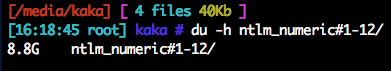
\includegraphics[scale=1]{5-1.png}
\caption{优化后彩虹表的空间大小}
\label{fig:5.1}
\end{figure}

新的彩虹链的数据结构实现如下,在以后的测试实验中,我们将都采用这种优化过的彩虹表。
\begin{lstlisting}
struct RTCFileHeader
{
    unsigned int   uVersion;    
    unsigned short uIndexSBits; 
    unsigned short uIndexEBits; 
    uint64         uIndexSMin;
    uint64         uIndexEMin;
    uint64         uIndexEInterval;
};
\end{lstlisting}

在存储上,除了对表的大小进行优化,还可以对系统的储存架构进行优化。在文件系统上,我们采用先进的XFS文件系统,XFS是由Silico Graphics,Inc.于90年代初开发的,它采用了优化算法,对查询分配存储空间非常快,可以支持上百万T字节的存储空间,特别是对大文件的支持表现相当出众;XFS采用B+树结构保证文件系统可以快速搜索于空间分配;XFS几乎以接近裸设备I/O的性能存储数据,在单个文件系统测试种,其吞吐量可高达7GB每秒,对单个文件的读写操作,其吞吐量可达4GB每秒。基于XFS以上特性,正符合彩虹表多个大文件读取的特点,下图为XFS与EXT3、EXT4的性能比较:
\begin{figure}[!ht]
\centering
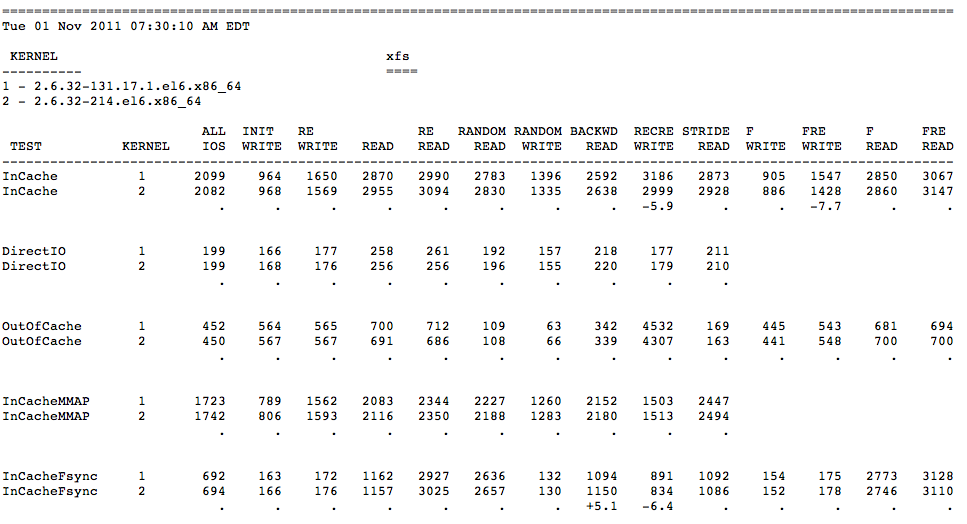
\includegraphics[scale=0.35]{5-2.png}
\caption{XFS性能测试}
\label{fig:5.2}
\end{figure}
\begin{figure}[!ht]
\centering
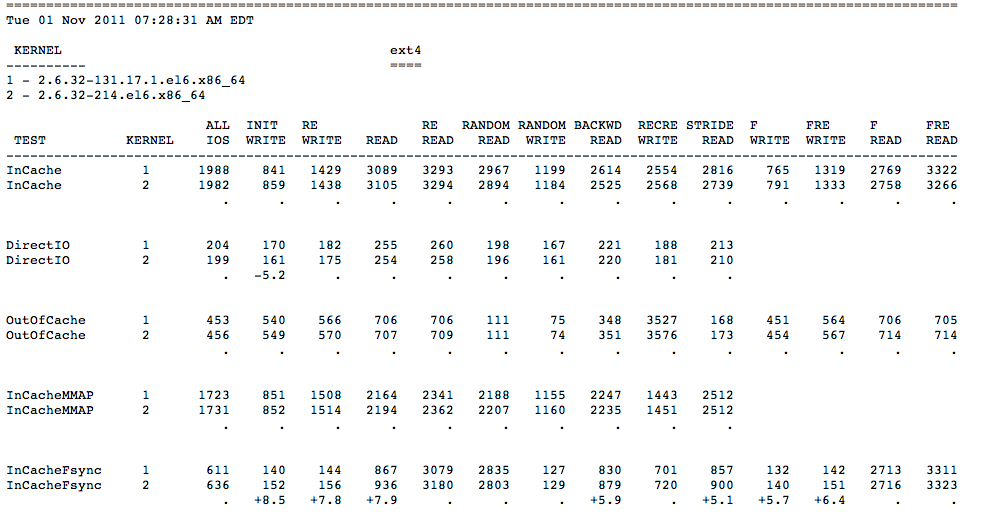
\includegraphics[scale=0.35]{5-3.png}
\caption{EXT4性能测试}
\end{figure}
\begin{figure}[!ht]
\centering
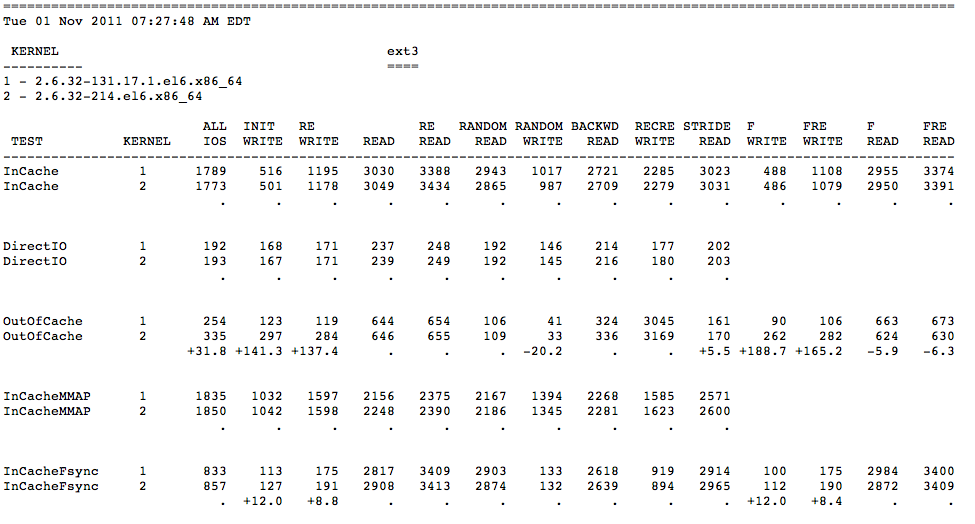
\includegraphics[scale=0.35]{5-4.png}
\caption{EXT3性能测试}
\end{figure}

从这3组性能测试数据我们可以看出XFS在大多数的的选项上要优于EXT4和EXT3,特别是在大文件的读取上。

接着是对存储硬件升级,这里我们主要升级的是硬盘,下表\ref{tab:5.1}是我们对不同配置硬盘的读速度进行数据对比,从表中可以明显看出使用SSD硬盘RAID0阵列后,读取速度将比一块7200转的硬盘提升了10倍,这将大大缩小破解的实际时间。最后的需要升级的系统内存,我们知道在计算机存储体系结构中,内存的读取速度要比硬盘快上许多倍,在Linux系统上内存以/dev/shm/设备呈现给用户,用户可以对次进行读写操作。

往后我们还可以采用iSCSI网络存储结构,iSCSI技术一种优IBM公司研究开发的,是一种新存储技术,可是实现在IP网络上运行SCSI协议,使其能在高速千兆或万兆以太网上进行网络传输。再加上FCoE技术,可以达到几Gb/s的存储速度。
\begin{longtable}{@{\extracolsep{\fill}}ccc}
\caption{各种存储系统读速度对比数据}\\\toprule[1pt]
\multicolumn{1}{c}{硬盘配置} & 
\multicolumn{1}{c}{读速度(hdparm -t)} &
\multicolumn{1}{c}{索引速度} \\\midrule
1x Maxtor 6B250S0 7200 RPM & 54MB/s & 640h/s \\
6x Seagate ST31500341AS 7200 RPM (RAID6) & 390MB/s & 4375h/s \\
2x APPLE SSD SM128C (RAID0) & 522MB/s & 6120h/s \\
\bottomrule[1pt]
\label{tab:5.1}
\end{longtable}

\section{算法结构优化}
密钥明文字符集被预计算成hash密文并和明文成对地储存在彩虹链中,如果要破解的hash密文在我们之前生成好的彩虹链中,则破解成功,反之破解失败。彩虹链存储的“明文-密文”对数量随着链表长度(t)的增加而增加,然而这些彩虹链会产生冲突,主要由于减约函数并不是一一对应的。图\ref{fig:5.5}示意了冲突的过程,最后这两条链表会合并成一条。
\begin{figure}[!ht]
\centering
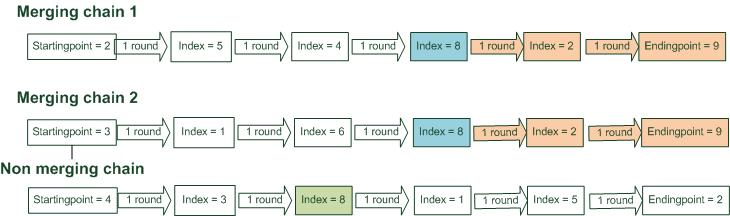
\includegraphics[scale=0.7]{5-5}
\caption{链表合并过程示意图}
\label{fig:5.5}
\end{figure}

无冲突的彩虹链个数会随着彩虹表的长度增加而减少,根据公式\eqref{equ:3.13},利用matlab软件我们可以得到关系图\ref{fig:5.6}。
\begin{figure}[!ht]
\centering
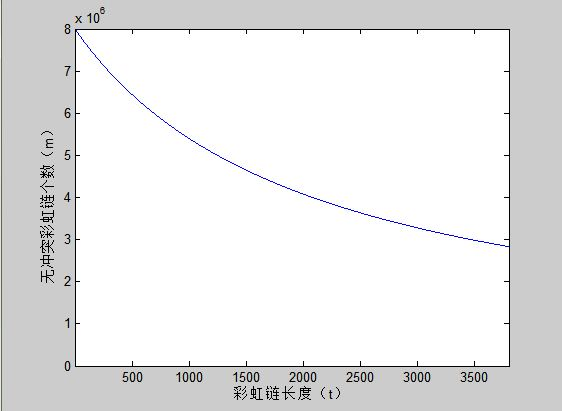
\includegraphics[scale=0.5]{5-6}
\caption{无冲突链表数-链表长度关系}
\label{fig:5.6}
\end{figure}

接着我们来分析表的张数(参数l)对破解成功概率的影响,我们把破解成功率公式\eqref{equ:3.13}在matlab下的实现函数为:\\
demo\_advantage\_of\_multiple\_table(),具体的函数实现可以参考附录A1.2。我们用不同的曲线表示当硬盘空间增大的情况下,破解的成功概率会随之增加,图\ref{fig:5.7}有5条曲线,分别表示彩虹表张数为1\~5时,破解的成功率和硬盘空间之间的关系,放大后,我们可以看出彩虹表的张数越多,曲线越快接近100\%,也就是在其他参数不变的情况下,增加参数l(彩虹表张数),可以得到越高破解成功概率;但也不是生成的彩虹表张数越多越好,当随着彩虹表的增加,我们需要在存储空间也就越大,这样会破解实际所消耗的时间就会增加,反而适得其反,所以时空折中算法的精髓就在于对时间和空间的代价进行不断地平衡,找出一个折中的代价。
\begin{figure}[!h]
\begin{floatrow}
\ffigbox{\caption{5张彩虹表的破解成功率}}{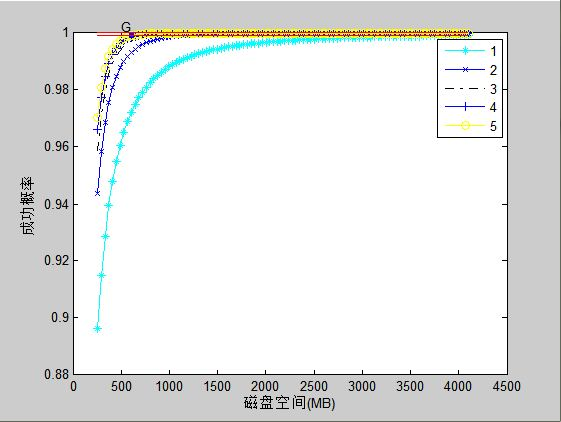
\includegraphics[scale=0.35]{5-7}}
\ffigbox{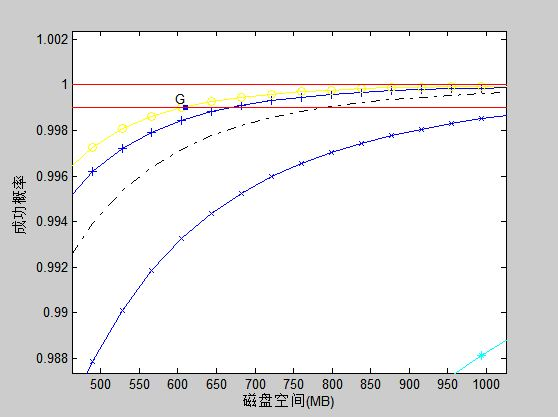
\includegraphics[scale=0.35]{5-8}}{\caption{5张彩虹表的破解成功率(放大)}}
\end{floatrow}
\end{figure}
\section{本文的实现与性能分析}
\section{本章小结}
本章对从计算能力到存储和彩虹表算法结构三方面进行优化和实现。在计算能力上我们提出了基于CUDA和云计算两种优化方法,并实现了CUDA GPU方案,从实际实验结果验证了这一设计方案;在存储系统上,我们提出了采用新型的彩虹表结构体,减少了彩虹表的磁盘存储空间,优化升级了物理的存储设备,在破解时间上得到了很好的提升;在彩虹表算法参数上,我们进行数据分析,优化了算法的参数。

\begin{figure}[!h]
\begin{floatrow}
\ffigbox{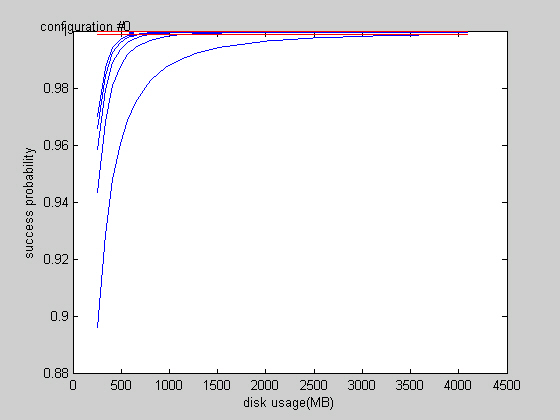
\includegraphics[scale=0.35]{5-9}}{\caption{总表空间大小-成功率关系图}}
\ffigbox{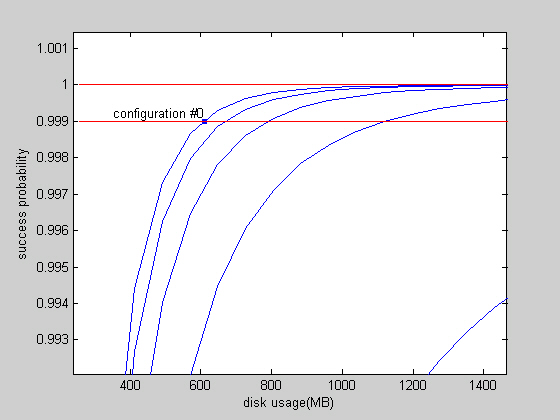
\includegraphics[scale=0.35]{5-10}}{\caption{总表空间大小-成功率关系图(放大)}}
\end{floatrow}
\end{figure}

